% Template for Cogsci submission with R Markdown

% Stuff changed from original Markdown PLOS Template
\documentclass[10pt, letterpaper]{article}

\usepackage{cogsci}
\usepackage{pslatex}
\usepackage{float}
\usepackage{caption}

% amsmath package, useful for mathematical formulas
\usepackage{amsmath}

% amssymb package, useful for mathematical symbols
\usepackage{amssymb}

% hyperref package, useful for hyperlinks
\usepackage{hyperref}

% graphicx package, useful for including eps and pdf graphics
% include graphics with the command \includegraphics
\usepackage{graphicx}

% Sweave(-like)
\usepackage{fancyvrb}
\DefineVerbatimEnvironment{Sinput}{Verbatim}{fontshape=sl}
\DefineVerbatimEnvironment{Soutput}{Verbatim}{}
\DefineVerbatimEnvironment{Scode}{Verbatim}{fontshape=sl}
\newenvironment{Schunk}{}{}
\DefineVerbatimEnvironment{Code}{Verbatim}{}
\DefineVerbatimEnvironment{CodeInput}{Verbatim}{fontshape=sl}
\DefineVerbatimEnvironment{CodeOutput}{Verbatim}{}
\newenvironment{CodeChunk}{}{}

% cite package, to clean up citations in the main text. Do not remove.
\usepackage{apacite}

% KM added 1/4/18 to allow control of blind submission
\cogscifinalcopy

\usepackage{color}

% Use doublespacing - comment out for single spacing
%\usepackage{setspace}
%\doublespacing


% % Text layout
% \topmargin 0.0cm
% \oddsidemargin 0.5cm
% \evensidemargin 0.5cm
% \textwidth 16cm
% \textheight 21cm

\title{Title TBD}


\author{Kennedy Casey \\
        University of Chicago \\
        \texttt{kbcasey@uchicago.edu}
\And \textbf{Elizabeth Mickiewicz} \\
             University of Chicago \\
             \texttt{lizmick9@uchicago.edu}
\And \textbf{Kimberly Shorter} \\
             University of Chicago \\
             \texttt{klshorter@uchicago.edu}
\And \textbf{Anapaula Silva Mandujano} \\
             University of Chicago \\
             \texttt{anapaula@uchicago.edu}            
\AND \textbf{Mara Duquette} \\
             University of Chicago \\
             \texttt{duquettemara@uchicago.edu}
\And \textbf{Mary Elliott} \\
             University of Texas at Dallas \\
             \texttt{maryle18@gmail.com}
\And \textbf{Elika Bergelson} \\
             Duke University \\
             \texttt{elika.bergelson@duke.edu}
\And \textbf{Marisa Casillas} \\
             University of Chicago \\
             \texttt{mcasillas@uchicago.edu}}


\begin{document}

\maketitle

\begin{abstract}


\textbf{Keywords:}

\end{abstract}

\hypertarget{introduction}{%
\section{Introduction}\label{introduction}}

The artifacts of everyday life reflect our routines, aspirations,
relationships, and much more. In particular, the objects that we
regularly pick up and handle---a coffee cup, a laptop, a baby
bottle---offer a window into the physical, social, and cultural contexts
that shape our understanding of the world. In this paper, we explore
patterns in object handling as a glimpse into everyday life at its
roots, from early infancy until age four.

For young learners, objects and their associated activities form a
critical source of input for social learning, including the ways in
which children are exposed to language relating to those objects
(yu/smithetc REFS; see also (\textbf{herzberg2021infant?}) for an
overview of object play and motor learning). This object-centered input
changes enormously across the first few years due to both maturational
constraints and culture-specific caregiving practices. In early infancy,
children have little ability to hold things or to control their posture,
primarily experiencing objects through what others bring near to them
(faces may make up a much greater proportion of their social input at
this point; fauseyREF). However, later gains in manual dexterity and
gross motor skill (e.g., sitting, crawling, walking) increasingly widen
their ability to seek, reach, and grab a diversity of objects in their
environment and give them greater control over what they handle, how,
and for how long (REFS).

Separately, access to objects is shaped by culture-specific practices
for carrying children, keeping them safe and warm, and scaffolding the
development of valued capacities (e.g., word learning in many US
families, walking in Kenyan Kipsigis families,
(\textbf{super1976environmental?})), all of which may slightly alter the
course of motor development (see (\textbf{adolph2010motor?}) for an
overview).

The array of objects available to children will also vary
crossculturally, including: (a) objects spread via globalization (e.g.,
plastic bags), (b) objects that have a basic functional role that is
similar across many contexts (e.g., spoon-like things for eating), and
(c) objects are specific to people and places (e.g., the gourd and
bombilla for drinking mate in much of South America, stemming from
Guaraní and Tupí tradition). Take, for example, middle-class US family
homes, which have been noted for their large quantities of possessions
(``clutter''), much of which is designed specifically for children
(e.g., toys and books (\textbf{arnold2017life?})). We might infer based
on this distribution of objects that much of what children do and talk
about at home is tailored to what particularly interests them and thus
children's worlds, in this sense, look very different from adults'.
Recent work by Herzberg and colleagues (\textbf{herzberg2021infant?})
underscores this point; their study of object play in 13--23-month-olds
showed that infants spent nearly 70\% of their time with toys or a mix
of toys and non-toys, with \textasciitilde100\% of infants playing with
children's books and stuffed animals and a total of 32 toy types
appearing in \(\ge\) 25\% of infants' play. Non-toy play was also
common, but still appeared to predominantly include infant-specific
objects (e.g., sippy cups, baby spoons, high chairs, pacifiers). We
would expect many of these items to be rare in other parts of the world,
with much greater overlap between objects for infants and objects for
adults (e.g., (\textbf{karasik2018not?})).

\hypertarget{methods}{%
\section{Methods}\label{methods}}

\hypertarget{corpus}{%
\subsection{Corpus}\label{corpus}}

\hypertarget{manual-annotation}{%
\subsection{Manual annotation}\label{manual-annotation}}

\hypertarget{reliability}{%
\subsection{Reliability}\label{reliability}}

\begin{table}[!ht]
\centering
\begingroup\small
\begin{tabular}{lll}
  \hline
Object Category & Rossel & Tseltal \\ 
  \hline
Synthetic & rope, shirt, plastic bottle & shirt, chair, pants \\ 
  Food & coconut, betelnut, tuber & guava, tortilla, apple \\ 
  Tool & knife, bowl, spoon & bowl, cup, bottle \\ 
  Toy & ball, book, plastic toy & book, toy truck, baby doll \\ 
  Natural & stick, rock, leaf & stick, leaf, tree \\ 
  Immovable & veranda, ladder, railing & door, fence, table \\ 
   \hline
\end{tabular}
\endgroup
\caption{Objects handled by the most children across categories and sites.} 
\end{table}

\hypertarget{results}{%
\section{Results}\label{results}}

\hypertarget{overall-frequency-statistics}{%
\subsection{Overall frequency
statistics}\label{overall-frequency-statistics}}

Children handled an average of 21.16 unique objects per day (median =
20, \emph{SD} = 15.2, range = 1--59), with no significant differences
across sites (\emph{M}\textsubscript{\emph{Rossel}} = 18.93,
\emph{M}\textsubscript{\emph{Tseltal}} = 23.24, \emph{W} = 350, \emph{p}
= 0.501). Only 20.83\% of objects were present in both communities, but
several shared objects were among the most frequently handled by
children in both sites. In fact, among the top 25 most common objects,
11 were shared across sites.

The frequency of object categories was similarly divided across sites
(Figure 1A). The top objects for each category are shown in Table 1.
Children primarily handled miscellaneous synthetic objects (e.g., rope,
guitar, shirt, etc.; \emph{M}\textsubscript{\emph{Rossel}} = 32.01\% of
handling, \emph{M}\textsubscript{\emph{Tseltal}} = 37.5\%) and food
(\emph{M}\textsubscript{\emph{Rossel}} = 28.58\%,
\emph{M}\textsubscript{\emph{Tseltal}} = 36.21\%). For 45 of 56
children, the top category was either synthetic objects or food.
Two-tailed Wilcoxon tests revealed only one significant category-level
difference between sites: children's handling of large or immovable
objects (e.g., veranda, ladder, railing, etc.), where Rossel children
handled these objects more frequently than Tseltal children
(\emph{M}\textsubscript{\emph{Rossel}} = 7.73\%,
\emph{M}\textsubscript{\emph{Tseltal}} = 3.31\%, adjusted \emph{p} =
0.038, \emph{p}s for all other categories \textgreater{} 0.05), but
these objects were still the least frequently handled in both sites.

During any given hour, children handled 5.26 objects from 2.79 different
categories, on average (median = 4.5 objects, \emph{SD} = 3.92, range =
1--18). A linear mixed-effects model with fixed effects of site, each of
6 object categories, and their interaction showed a significant main
effect of the synthetic object category (\(\beta\) = 0.52, \emph{SE} =
0.2, \emph{t} = 2.59, \emph{p} = 0.01) as well as an interaction between
site and the synthetic object category (\(\beta\) = 1.11, \emph{SE} =
0.29, \emph{t} = 3.88, \emph{p} = \textless{} 0.001) such that children
handled more unique synthetic objects per hour than any other object
category, and this effect was stronger for Tseltal children than for
Rossel children (\emph{p}s \textgreater{} 0.05 for all other main
effects and interaction terms; Figure 1B).

\begin{CodeChunk}
\begin{figure}[!ht]

{\centering 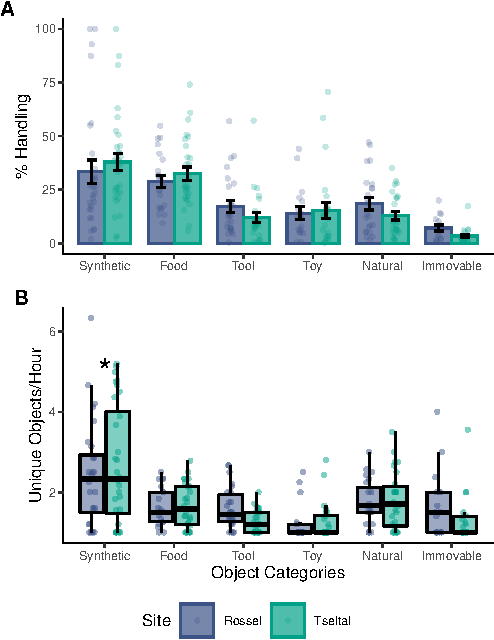
\includegraphics{figs/overall-stats-fig-1} 

}

\caption[(A) Overall frequency of handling by object category]{(A) Overall frequency of handling by object category. Points reflect percentages for individual children. (B) Count of unique objects handled per hour by object category. Points reflect means for individual children across all hours of recording.}\label{fig:overall-stats-fig}
\end{figure}
\end{CodeChunk}

\hypertarget{time-of-day-effects}{%
\subsection{Time of day effects}\label{time-of-day-effects}}

Children's overall rate of object handling was largely consistent across
the day. The number of unique handled objects per hour was not linearly
related to time of day (\(\beta\) = -0.02, \emph{SE} = 0.11, \emph{t} =
-0.16, \emph{p} = 0.874), and there was no two-way interaction between
time of day and site (\(\beta\) = 0.01, \emph{SE} = 0.14, \emph{t} =
0.1, \emph{p} = 0.923).

However, we did find differences in children's rates of holding for
specific object categories across the day. We ran individual linear
mixed-effects models, which included fixed effects of site, hour of the
day, and their interaction, for each of 6 categories. Synthetic objects
were marginally more common during the afternoon hours (\(\beta\) =
0.02, \emph{SE} = 0.01, \emph{t} = 1.71, \emph{p} = 0.09), and food
items were handled with significantly greater frequency during the
morning hours (\(\beta\) = -0.03, \emph{SE} = 0.01, \emph{t} = -2.76,
\emph{p} = 0.006; Figure 2). No other main effects or two-way
interactions reached statistical significance (all \emph{p}s
\textgreater{} 0.05).

\begin{CodeChunk}
\begin{figure}[!ht]

{\centering 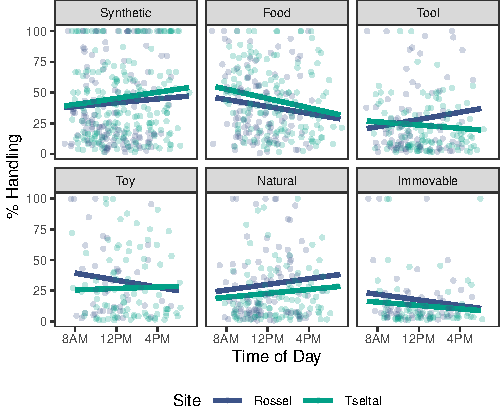
\includegraphics{figs/tod-effects-fig-1} 

}

\caption[Frequency of handling by object category across different times of day]{Frequency of handling by object category across different times of day. Individual points show raw percentages for each child, and lines reflect model-predicted percentages.}\label{fig:tod-effects-fig}
\end{figure}
\end{CodeChunk}

\hypertarget{age-effects}{%
\subsection{Age effects}\label{age-effects}}

Children's overall rate of object handling increased marginally with age
(Figure 3A). That is, older children handled more unique objects per
hour (\(\beta\) = 0.07, \emph{SE} = 0.03, \emph{t} = 1.99, \emph{p} =
0.05). Additionally, with increasing age, children handled more objects
from different categories per hour (\(\beta\) = 0.03, \emph{SE} = 0.01,
\emph{t} = 2.6, \emph{p} = 0.011). These effects were consistent across
sites; we found no main effects of site or interactions between site and
age (all \emph{p}s \textgreater{} 0.05).

\begin{CodeChunk}
\begin{figure}[!ht]

{\centering 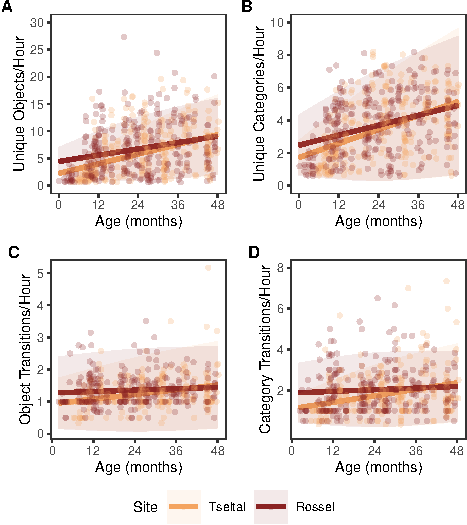
\includegraphics{figs/age-effects-fig-1} 

}

\caption[(A) Unique objects and (B) object categories handled per hour as a function of age]{(A) Unique objects and (B) object categories handled per hour as a function of age. Points reflect raw hourly counts for each child, and lines reflect model predictions with shaded standard error regions.}\label{fig:age-effects-fig}
\end{figure}
\end{CodeChunk}

\hypertarget{discussion}{%
\section{Discussion}\label{discussion}}

\hypertarget{references}{%
\section{References}\label{references}}

\setlength{\parindent}{-0.1in} 
\setlength{\leftskip}{0.125in}

\noindent

\bibliographystyle{apacite}


\end{document}
